\section{Microfono: implementación de filtro de segundo orden}
\begin{frame}
\frametitle{Filtro de segundo orden en el micrófono}
Se decidió implementar un filtro de segundo orden para lograr una mejor atenuación de la onda a frecuencias cercanas a los $2kHz$.
\begin{figure}[H]
			\centering
			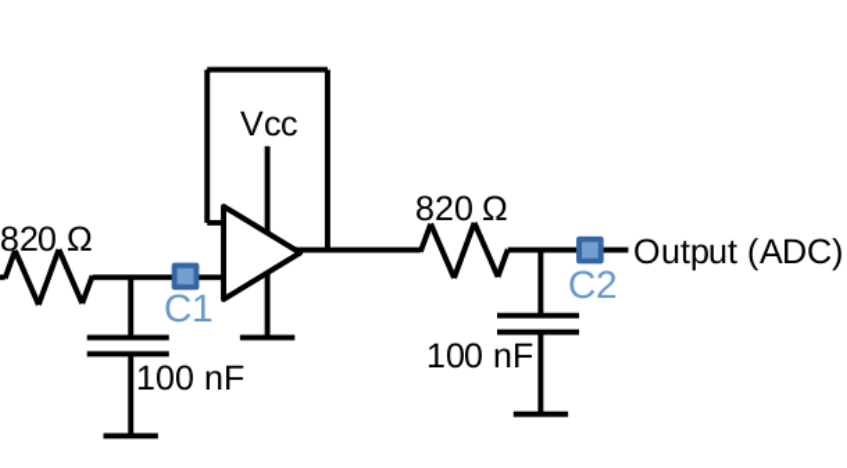
\includegraphics[scale=0.3]{esqfiltro}
			\caption{Esquema del filtro implementado en la salida del micrófono}	
		\end{figure}
\end{frame}



\begin{frame}
\frametitle{Filtro de segundo orden:Gráfico}
\begin{columns}[t]
		\column{0.5\textwidth}
		\begin{figure}[H]
			\centering
			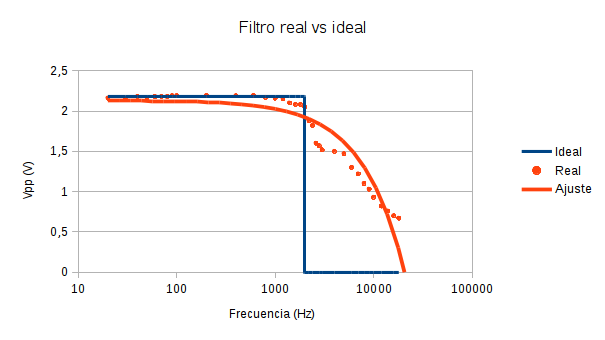
\includegraphics[scale=0.3]{Graf}
			\caption{Gráfico de la respuesta de tensión en función de la frecuencia para un filtro de \emph{primer} orden}	
		\end{figure}
		\column{0.5\textwidth}
		\begin{figure}[H]
			\centering
			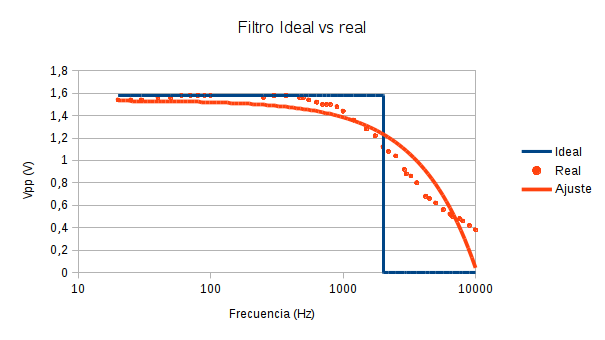
\includegraphics[scale=0.3]{Graf2do}
			\caption{Gráfico de la respuesta de tensión en función de la frecuencia para un filtro de \emph{segundo} orden}	
		\end{figure}
	\end{columns}
2\end{frame}